The preceding section described \emph{how} RECTOR selects a trajectory: the applicability head, proxy evaluation, and lexicographic scorer operate on rule-level violation severities and applicability masks.  This section specifies \emph{what} those rules are and \emph{how} their violations are computed---operationalizing the prioritized rulebook into 28~rules across four tiers, with differentiable smooth proxies for 24 of them.

Each tier has a distinct proxy design rationale.  \textbf{Tier~0 (Safety, 5~rules)} focuses on collision avoidance and minimum clearance: collision avoidance~(L0.R3) is approximated using a differentiable SAT-based oriented-bounding-box~(OBB) penetration-depth proxy.  \textbf{Tier~1 (Legal, 7~rules)} encodes traffic laws such as signal compliance and right-of-way; proxies shift from geometric distances to event-based detectors---for instance, Red Light Stop~(L1.R3) penalises crossing a stop line when the signal state is red. \textbf{Tier~2 (Road, 2~rules)} enforces drivable-surface and lane-keeping constraints using signed distance functions~(SDFs) to road polygons. \textbf{Tier~3 (Comfort, 14~rules)} enforces bounds on acceleration, jerk, and steering to maintain ride quality.

To maintain rigour, we apply the \emph{Evaluation Dual-Protocol} introduced in Section~\ref{subsec:fullcatalog_context}: (i)~\emph{Protocol~A} uses 24~proxied rules with predicted applicability for training and selection, and (ii)~\emph{Protocol~B} applies the full 28-rule Waymo evaluator with oracle applicability for reporting and verification.  This allows \textsc{RECTOR} to be trained on continuous differentiable signals while being audited against the absolute standards of the full rule catalog.

%-------------------------------------------------------------------------------
\subsection{Rule Catalog Overview}
\label{subsec:rule_catalog}
%-------------------------------------------------------------------------------

The rule catalog comprises 28~rules organized into four tiers consistent with the priority structure formalized in Section~\ref{Sec:Problem_Formulation}.  Tier~0 (Safety) captures physical safety and collision avoidance; Tier~1 (Legal) captures rules derived from traffic-law concepts in the WOMD annotation framework;\footnote{See the Legal-tier disclaimer in Section~\ref{subsec:observations}.} Tier~2 (Road) captures drivable-surface and lane-keeping constraints; and Tier~3 (Comfort) captures ride quality and context policies. Table~\ref{tab:rule_catalog} lists the complete catalog used in all experiments.

\noindent\textbf{Rule ID convention.}  We denote rules as $\mathrm{L}\ell.\mathrm{R}i$, where $\ell$ is the priority \emph{level} index (smaller~$\ell$ indicates higher priority) and $i$ enumerates rules within that level; the \emph{Tier} column groups levels into the four coarse tiers used throughout the paper.

\begin{table*}[h]
\centering
\caption{Complete Rule Catalog with Tier Assignments (28 Rules)}
\label{tab:rule_catalog}
\small
\begin{tabular}{llp{4.5cm}p{3.5cm}}
\toprule
\textbf{Rule ID} & \textbf{Tier} & \textbf{Description} & \textbf{Waymo Module}$^\ddagger$ \\
\midrule
\multicolumn{4}{l}{\textit{Tier 0: Safety (5 rules)}} \\
L0.R0 & Safety & Safe longitudinal distance & \texttt{\footnotesize l0\_safe\_long\_dist} \\
L0.R1 & Safety & Safe lateral clearance & \texttt{\footnotesize l0\_safe\_lat\_clear} \\
L0.R2 & Safety & Crosswalk occupancy & \texttt{\footnotesize l0\_crosswalk\_occ} \\
L0.R3 & Safety & Collision avoidance (overlap) & \texttt{\footnotesize l10\_collision} \\
L0.R4 & Safety & VRU clearance buffer & \texttt{\footnotesize l10\_vru\_clearance} \\
\midrule
\multicolumn{4}{l}{\textit{Tier 1: Legal (7 rules)}} \\
L1.R0 & Legal & Traffic signal compliance & \texttt{\footnotesize l5\_signal\_compliance} \\
L1.R1 & Legal & Priority / right-of-way & \texttt{\footnotesize l5\_priority\_viol} \\
L1.R2 & Legal & Speed limit adherence & \texttt{\footnotesize l07\_speed\_limit} \\
L1.R3 & Legal & Red light stop compliance & \texttt{\footnotesize l8\_red\_light} \\
L1.R4 & Legal & Stop sign compliance & \texttt{\footnotesize l08\_stop\_sign} \\
L1.R5 & Legal & Crosswalk yield to pedestrians & \texttt{\footnotesize l08\_crosswalk\_yield} \\
L1.R6 & Legal & Wrong-way driving prevention & \texttt{\footnotesize l08\_wrongway} \\
\midrule
\multicolumn{4}{l}{\textit{Tier 2: Road (2 rules)}} \\
L2.R0 & Road & Drivable surface constraint & \texttt{\footnotesize l3\_drivable\_surface} \\
L2.R1 & Road & Lane departure prevention & \texttt{\footnotesize l07\_lane\_departure} \\
\midrule
\multicolumn{4}{l}{\textit{Tier 3: Comfort (14 rules)}} \\
L3.R0 & Comfort & Smooth longitudinal acceleration & \texttt{\footnotesize l1\_smooth\_accel} \\
L3.R1 & Comfort & Smooth braking deceleration & \texttt{\footnotesize l1\_smooth\_braking} \\
L3.R2 & Comfort & Smooth lateral steering & \texttt{\footnotesize l1\_smooth\_steering} \\
L3.R3 & Comfort & Speed consistency & \texttt{\footnotesize l1\_speed\_consistency} \\
L3.R4 & Comfort & Jerk / lane-change smoothness & \texttt{\footnotesize l1\_lane\_change\_smooth} \\
L3.R5 & Comfort & Left turn gap acceptance & \texttt{\footnotesize l4\_left\_turn\_gap} \\
L3.R6 & Comfort & Parking zone violation & \texttt{\footnotesize l5\_parking\_viol} \\
L3.R7 & Comfort & School zone speed compliance & \texttt{\footnotesize l5\_school\_zone} \\
L3.R8 & Comfort & Construction zone compliance & \texttt{\footnotesize l5\_construction\_zone} \\
L3.R9 & Comfort & Cooperative lane change & \texttt{\footnotesize l6\_coop\_lane\_change} \\
L3.R10 & Comfort & Safe following distance & \texttt{\footnotesize l6\_following\_dist} \\
L3.R11 & Comfort & Intersection negotiation & \texttt{\footnotesize l6\_intersection\_neg} \\
L3.R12 & Comfort & Pedestrian interaction & \texttt{\footnotesize l6\_pedestrian\_inter} \\
L3.R13 & Comfort & Cyclist interaction & \texttt{\footnotesize l6\_cyclist\_inter} \\
\bottomrule
\end{tabular}
\vspace{1mm}
\caption*{\footnotesize 86\% of rules (24/28) have differentiable proxy implementations. The remaining 14\% require intent modeling, counterfactual scene reasoning, or multi-agent negotiation and are handled via conservative applicability defaults. See Section~\ref{subsec:proxy_functions}. $^\ddagger$\textbf{Waymo Module} gives the Python module name in the \texttt{waymo\_rule\_eval/rules/} package of the evaluation codebase.  Figures reporting per-rule statistics (Figs.\ \ref{fig:rule_breakdown} and \ref{fig:per_rule_heatmap}) use shortened bar labels derived from these module names. The paper's \texttt{L\textit{i}.R\textit{j}} identifiers use a sequential within-tier enumeration; the canonical registry IDs in \texttt{waymo\_rule\_eval/rules/registry.py} differ because they follow the original Waymo rulebook numbering.  The complete mapping is: \textbf{Safety}---L0.R0$\!\to$\texttt{L0.R2}, L0.R1$\!\to$\texttt{L0.R3}, L0.R2$\!\to$\texttt{L0.R4}, L0.R3$\!\to$\texttt{L10.R1}, L0.R4$\!\to$\texttt{L10.R2}; \textbf{Legal}---L1.R0$\!\to$\texttt{L5.R1}, L1.R1$\!\to$\texttt{L5.R2}, L1.R2$\!\to$\texttt{L7.R4}, L1.R3$\!\to$\texttt{L8.R1}, L1.R4$\!\to$\texttt{L8.R2}, L1.R5$\!\to$\texttt{L8.R3}, L1.R6$\!\to$\texttt{L8.R5}; \textbf{Road}---L2.R0$\!\to$\texttt{L3.R3}, L2.R1$\!\to$\texttt{L7.R3}; \textbf{Comfort}---L3.R0--R4$\!\to$\texttt{L1.R1--R5}, L3.R5$\!\to$\texttt{L4.R3}, L3.R6--R8$\!\to$\texttt{L5.R3--R5}, L3.R9--R13$\!\to$\texttt{L6.R1--R5}.}
\end{table*}

%-------------------------------------------------------------------------------
\subsection{Per-Rule Applicability Analysis}
\label{subsec:per_rule_analysis}
%-------------------------------------------------------------------------------

Fig.~\ref{fig:rule_breakdown} reports per-rule applicability F1 by tier on a diagnostic sample. The figure is used later to localize where the learned applicability head fails; the deployment-facing conclusion that conservative activation is preferable is supported by the full-split cross-evaluation in Section~\ref{Sec:Accuracy_SectionRule-Compliance_Behavior_and_Efficiency}, not by this figure alone.

\begin{figure*}
\centering
\begin{subfigure}[t]{0.48\textwidth}
\centering
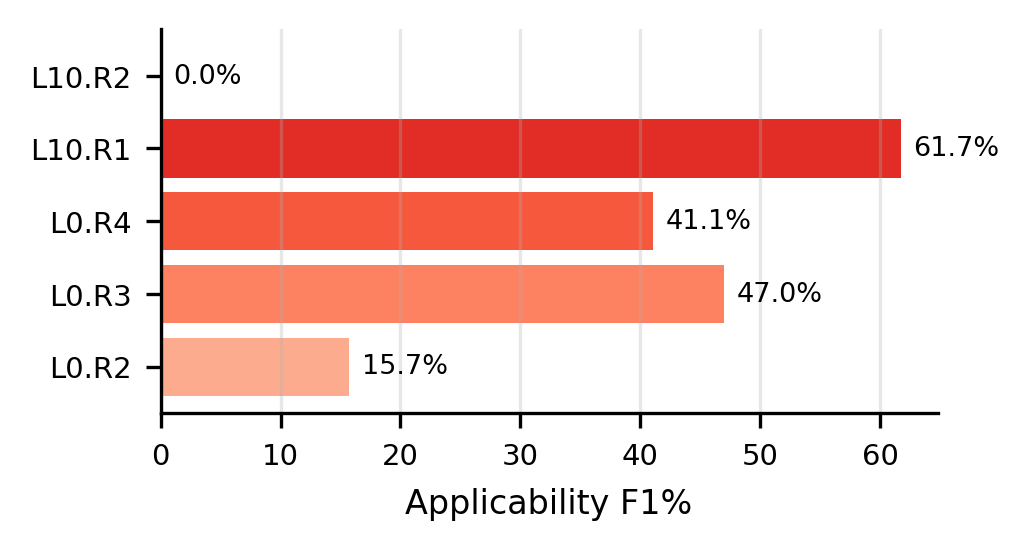
\includegraphics[width=\textwidth]{Figures/rule_breakdown_a.png}
\caption{Tier~0 (Safety)}
\end{subfigure}
\hfill
\begin{subfigure}[t]{0.48\textwidth}
\centering
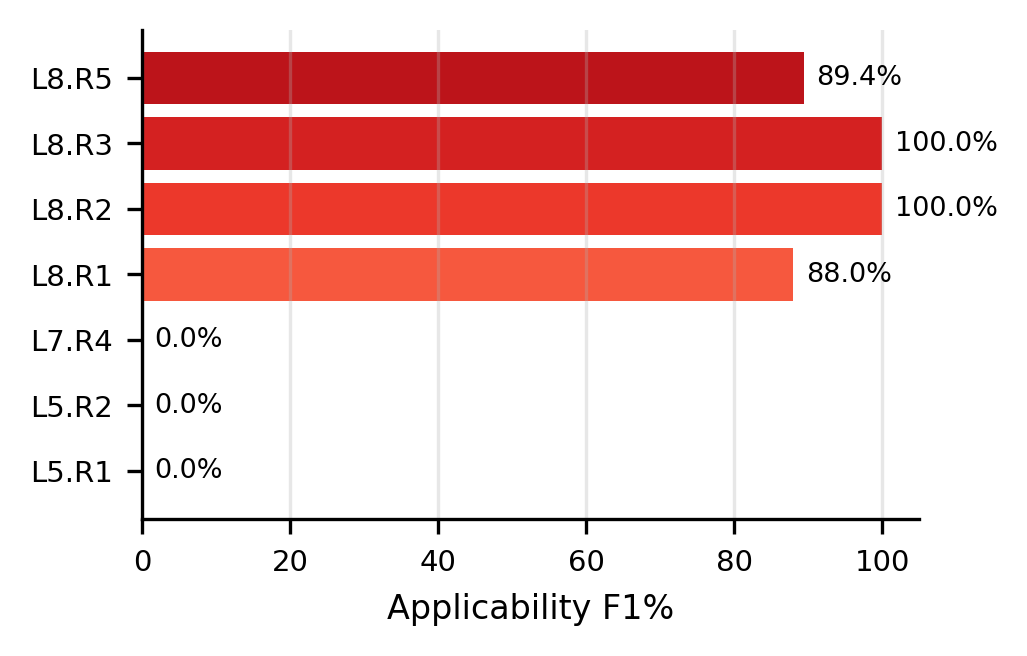
\includegraphics[width=\textwidth]{Figures/rule_breakdown_b.png}
\caption{Tier~1 (Legal)}
\end{subfigure}
\caption{Per-rule applicability F1 scores for RECTOR predictions (WOMD v1.3.0 \texttt{validation\_interactive}, 500~GT / 337~RECTOR scenarios), grouped by tier. Bar labels follow the Waymo evaluator's internal convention; the mapping to this paper's tier notation is given in Table~\ref{tab:rule_catalog}.}
\label{fig:rule_breakdown}
\end{figure*}

The observed support imbalance motivates the conservative applicability ablations in Section~\ref{Sec:Accuracy_SectionRule-Compliance_Behavior_and_Efficiency}.

%-------------------------------------------------------------------------------
\subsection{Waymo Rule Evaluation Framework}
\label{subsec:waymo_framework}
%-------------------------------------------------------------------------------

The per-rule analysis above relies on a ground-truth auditor that defines consistent rule semantics across scenarios.  We adopt the Waymo Open Motion Dataset rule evaluation framework in this role, because it provides (i)~standardised definitions for traffic-rule constraints, (ii)~consistent applicability semantics across scenarios, (iii)~comparability to prior WOMD-based methods, and (iv)~a stable baseline for regression tests when the model or proxies change.

\subsubsection{Map Feature Integration}

The evaluator relies on structured map elements: lane centre-lines and boundaries, stop lines, traffic signals, crosswalk polygons, and drivable-surface boundaries.  We extract these entities from the Waymo scenario protocol buffers and construct a compact, queryable representation used by both the full evaluator and the proxy layer (when available).

\subsubsection{Scenario Context Construction}

For each scenario, we build a context object that contains ego and agent trajectories, map features, signal states, and rule applicability metadata. During \emph{evaluation}, we use oracle applicability~$a_r^*$ derived from the scenario context and evaluate the complete 28-rule catalog.  During \emph{training and selection}, we evaluate only the proxy subset and use predicted applicability~$\hat{a}_r$ from Section~\ref{Sec:RECTOR}.  This separation prevents proxy limitations from silently altering audit metrics and ensures that the two protocols remain methodologically distinct as defined in Section~\ref{subsec:fullcatalog_context}.

%-------------------------------------------------------------------------------
\subsection{Smooth Proxy Functions}
\label{subsec:proxy_functions}
%-------------------------------------------------------------------------------

While the full evaluator provides the authoritative compliance verdict, it is non-differentiable and therefore cannot provide a gradient signal during training.  RECTOR therefore uses smooth proxy functions to (i)~support gradient flow for optional rule-shaped training losses (Section~\ref{subsec:training_objective}), and (ii)~produce stable, continuous severity values for tier aggregation at selection time.  Proxies approximate binary rule predicates with smooth penalties; while they cannot replicate every discrete semantic rule, they are sufficient to steer the generator away from recurrent geometric violations (e.g., clearance, lane departure, and speed).

\textbf{Proxy design principles.}  We convert thresholded predicates into smooth penalties using hinge-like terms $\max(0,\cdot)$ and soft indicator gates.  When a rule depends on an event (e.g., crossing a stop line), we approximate the event with a differentiable boundary function and a smooth difference across timesteps.  This yields informative gradients while keeping the proxy well-defined almost everywhere.

\subsubsection{Proxy Coverage}

Of the 28~cataloged rules, \textbf{24 have smooth proxy implementations}
(86\% coverage).  All Tier~0 (Safety) rules are covered, ensuring that the highest-priority constraints contribute a training signal. Table~\ref{tab:training_eval_comparison} summarizes the training versus evaluation protocol.

\begin{table}[h]
\centering
\caption{Training vs.\ Evaluation Comparison}
\label{tab:training_eval_comparison}
\begin{tabular}{lcc}
\toprule
\textbf{Aspect} & \textbf{Training} & \textbf{Evaluation} \\
\midrule
Rules evaluated & 24 (proxied) & 28 (all) \\
Applicability source & Predicted ($\hat{a}_r$) & Oracle ($a_r^*$) \\
Map context & Partial & Full \\
Gradient flow & Yes & No \\
Speed & Fast ($\sim$1\,ms) & Moderate ($\sim$5\,ms) \\
\bottomrule
\end{tabular}
\vspace{2mm}
\footnotesize
\textit{Note:} Training uses smooth proxies for 24/28 rules to provide a
gradient signal.  Evaluation uses the full Waymo framework with complete map
context for all 28 rules.
\end{table}

The four unproxied rules fall into two distinct categories. \textbf{L1.R1} (Priority/right-of-way) requires multi-agent intent modeling and counterfactual scene reasoning that cannot be reliably approximated with geometric operations alone.  The remaining three---\textbf{L3.R6}~(Parking zone), \textbf{L3.R7}~(School zone speed), and \textbf{L3.R8}~(Construction zone)---are computable from static map features in principle, but the WOMD~v1.3.0 interactive scenarios do not reliably include the corresponding zone polygon annotations; without polygon ground truth, a differentiable proxy cannot compute zone membership and is therefore omitted.  All four are handled via conservative applicability defaults in the selection pipeline and are included in the full-catalog evaluation (Protocol~B).

\subsubsection{Normalization of Proxy Severities}

Proxy outputs have heterogeneous units (e.g., metres, metres/second, IoU). To make tier aggregation well-defined, each proxy produces a raw severity~$V_r(\tau;s)\ge 0$ and a normalized severity~$\bar{V}_r(\tau;s)\in[0,1]$ via per-rule scaling and clamping:
\begin{equation}
\bar{V}_r(\tau;s)=\min\!\left(1,\,\frac{V_r(\tau;s)}{\alpha_r}\right),
\end{equation}
where $\alpha_r{>}0$ is the per-rule normalization constant introduced in Section~\ref{Sec:Problem_Formulation}.  In the released evaluator code this quantity appears as \texttt{RULE\_NORM} or \texttt{RULE\_NORMALIZATION}, so $\alpha_r \equiv V_r^{\max}$ in earlier drafts.  The tier aggregation and lexicographic scorer operate on~$\bar{V}_r$; the raw~$V_r$ is used in the training loss. This normalization contract is required by Proposition~\ref{thm:scalarization} to guarantee that the GPU-friendly scalarization preserves the lexicographic ordering.  Table~\ref{tab:proxy_constants} lists all per-rule proxy parameters.  In the released implementation, the linear normalization $\bar{V}_r = \min(1, V_r/\alpha_r)$ is replaced by an exponential cost function that maps raw violations to $[0,1]$ without a separate $\alpha_r$:
\begin{equation}
c_r(v) = 1 - \exp\!\bigl(-\kappa_r \cdot \max(0, v)\bigr),
\label{eq:exponential_cost}
\end{equation}
where $\kappa_r > 0$ is a per-proxy \emph{softness} parameter controlling how quickly the cost saturates.  This formulation satisfies the normalization contract (output in $[0,1]$, monotonically increasing in violation magnitude) required by Proposition~\ref{thm:scalarization}.

\begin{table*}[t]
\centering
\caption{Per-Rule Proxy Parameters: Softness Constants and Violation Thresholds}
\label{tab:proxy_constants}
\small
\setlength{\tabcolsep}{4pt}
\begin{tabular}{llccll}
\toprule
\textbf{Rule ID} & \textbf{Tier} & $\boldsymbol{\kappa_r}$ & \textbf{Threshold} & \textbf{Unit} & \textbf{Violation Semantics} \\
\midrule
\multicolumn{6}{l}{\textit{Tier 0: Safety}} \\
L0.R0 & Safety & 2.0 & 2.0 & m & Longitudinal gap $< d_{\min}$ to lead vehicle \\
L0.R1 & Safety & 2.0 & 0.5 & m & Lateral clearance $< d_{\text{lat}}$ to any agent \\
L0.R2 & Safety & 3.0 & 2.0 & m & Ego within crosswalk clearance zone \\
L0.R3 & Safety & 2.0 & 0.0 & m & OBB penetration depth (SAT) $> 0$ \\
L0.R4 & Safety & 2.0 & 1.0 & m & Distance to VRU $< d_{\text{VRU}}$ \\
\midrule
\multicolumn{6}{l}{\textit{Tier 1: Legal}} \\
L1.R0 & Legal & 3.0 & 2.0 & m & Crossing stop line under red signal \\
L1.R2 & Legal & 2.0 & --- & m/s & Speed $> v_{\text{limit}} + v_{\text{tol}}$ ($v_{\text{tol}}{=}$5\,mph) \\
L1.R3 & Legal & 3.0 & 2.0 & m & Crossing stop line under red signal \\
L1.R4 & Legal & 3.0 & 0.5 & m/s & Min speed in stop zone $> v_{\text{stop}}$ \\
L1.R5 & Legal & 3.0 & 5.0 & m & Ego within crosswalk yield radius \\
L1.R6 & Legal & 2.0 & 2.356 & rad & Heading deviation $>$ 135$^\circ$ from lane direction \\
\midrule
\multicolumn{6}{l}{\textit{Tier 2: Road}} \\
L2.R0 & Road & 2.0 & 1.0 & m & Signed distance outside drivable surface \\
L2.R1 & Road & 2.0 & 1.8 & m & Lateral offset $>$ half lane width $+$ margin \\
\midrule
\multicolumn{6}{l}{\textit{Tier 3: Comfort}} \\
L3.R0 & Comfort & 2.0 & 3.0 & m/s$^2$ & Longitudinal acceleration $> a_{\max}$ \\
L3.R1 & Comfort & 2.0 & 4.0 & m/s$^2$ & Braking deceleration $> a_{\text{brake}}$ \\
L3.R2 & Comfort & 2.0 & 0.5 & rad/s & Steering rate $> \omega_{\max}$ \\
L3.R3 & Comfort & 2.0 & 2.0 & m/s & Speed change $> \Delta v_{\max}$ \\
L3.R4 & Comfort & 2.0 & 2.0 & m/s$^3$ & Jerk $> j_{\max}$ \\
L3.R5 & Comfort & 2.0 & 4.0 & s & Left-turn TTC gap $< t_{\min}$ \\
L3.R9 & Comfort & 2.0 & 3.0 & s & Lane-change TTC $< t_{\min}$ \\
L3.R10 & Comfort & 2.0 & 2.0 & s & Following time $< t_{\text{follow}}$ \\
L3.R11 & Comfort & 2.0 & 3.0 & s & Intersection TTC $< t_{\min}$ \\
L3.R12 & Comfort & 2.0 & 3.0 & m & Pedestrian proximity $< d_{\text{VRU}}$ \\
L3.R13 & Comfort & 2.0 & 3.0 & m & Cyclist proximity $< d_{\text{VRU}}$ \\
\bottomrule
\end{tabular}
\vspace{1mm}
\caption*{\footnotesize $\kappa_r$: softness parameter in the exponential cost function (Eq.~\ref{eq:exponential_cost}).  Higher $\kappa_r$ causes faster saturation to maximum cost.  Signal-related proxies (L1.R0, L1.R3--R5, L0.R2) use $\kappa_r{=}3.0$; all others use $\kappa_r{=}2.0$.  Threshold: the physical limit above which the proxy begins to penalise; for rules where the threshold is inherent to the violation definition (e.g., speed limit), ``---'' indicates the threshold is scenario-dependent.  L1.R1 (priority), L3.R6--R8 (zone rules) are omitted as they lack proxy implementations.  Additional penalty scaling factors: yellow-light violations are scaled by 0.3$\times$, flashing-red by 0.5$\times$.}
\end{table*}
%-------------------------------------------------------------------------------
\subsection{Proxy Implementation Details}
\label{subsec:proxy_details}
%-------------------------------------------------------------------------------

We now present representative proxy formulations from each tier, ordered by priority.  All proxies are evaluated at $\Delta t = 0.1\,\mathrm{s}$ (10\,Hz); when a proxy depends on velocity, acceleration, jerk, or heading, we derive these quantities from the predicted trajectory by finite differences with standard endpoint handling.

\textbf{Notation.}  We use $\sigma_\alpha(x) = 1/(1{+}e^{-\alpha x})$ for sigmoid gates, and $\text{softmin}_\beta\{f_t\} = -\frac{1}{\beta}\log\sum_t e^{-\beta f_t}$ for smooth minimum approximation (with $\beta{=}10$).  The symbol $\alpha$ denotes a rule-specific gate sharpness parameter; the exact per-rule values are implementation constants rather than quantities tuned or compared in this paper.

\subsubsection{Safety Tier Proxies}

The Safety tier is the highest-priority tier, and all five of its rules have differentiable proxies.

For \textbf{L0.R0 (Safe Longitudinal Distance)}, we penalise insufficient longitudinal gap to the lead vehicle when the ego is moving:
\begin{equation}
V_{\text{L0.R0}}(\tau; s)=\sum_{t=1}^{T}\max\!\left(0,\,d_{\min}-d_t^{\text{long}}\right)\cdot \sigma_\alpha\!\left(\|\mathbf{v}_t\|-v_{\min}\right),
\end{equation}
where $d_t^{\text{long}}$ is the longitudinal distance to the lead vehicle, $d_{\min}{=}2.0\,\mathrm{m}$, and $v_{\min}{=}0.5\,\mathrm{m/s}$.

For \textbf{L0.R1 (Safe Lateral Clearance)}, we penalise lateral clearance violations to nearby agents:
\begin{equation}
V_{\text{L0.R1}}(\tau; s)=\sum_{t=1}^{T}\sum_{j\in\mathcal{A}_t}\max\!\left(0,\,d_{\text{lat}}-d_{t,j}^{\text{lat}}\right),
\end{equation}
where $d_{t,j}^{\text{lat}}$ is the lateral clearance between ego and agent~$j$ at time~$t$, and $d_{\text{lat}}{=}0.5\,\mathrm{m}$.

For \textbf{L0.R3 (Collision Avoidance)}, we use a differentiable Separating-Axis-Theorem~(SAT) penetration depth on axis-aligned oriented bounding boxes.  Given ego box half-extents $(l_{\text{ego}}/2,\,w_{\text{ego}}/2)$ and agent~$j$ half-extents $(l_j/2,\,w_j/2)$, we first rotate the relative displacement $\Delta\mathbf{p}_{t,j}=\tau_t^j-\tau_t$ into the ego frame via heading $\theta_t$:
\begin{equation}
\begin{pmatrix}\delta_{\text{long}}\\\delta_{\text{lat}}\end{pmatrix}
=
\begin{pmatrix}\cos\theta_t & \sin\theta_t\\-\sin\theta_t & \cos\theta_t\end{pmatrix}
\Delta\mathbf{p}_{t,j}.
\end{equation}
Per-axis penetration depths are then
\begin{align}
p_{\text{long}} &= \max\!\left(0,\;\tfrac{l_{\text{ego}}+l_j}{2}-|\delta_{\text{long}}|\right),\\
p_{\text{lat}}  &= \max\!\left(0,\;\tfrac{w_{\text{ego}}+w_j}{2}-|\delta_{\text{lat}}|\right),
\end{align}
and the SAT overlap depth (positive only when \emph{both} axes overlap) is $d_{t,j}=\min(p_{\text{long}},\,p_{\text{lat}})$.  The proxy cost is
\begin{equation}
V_{\text{L0.R3}}(\tau; s)=\sum_{t=1}^{T}\sum_{j\in\mathcal{A}_t}d_{t,j}.
\end{equation}

For \textbf{L0.R4 (VRU Clearance)}, we penalise proximity violations to pedestrians and cyclists:
\begin{equation}
V_{\text{L0.R4}}(\tau; s)=\sum_{t=1}^{T}\sum_{j\in\mathcal{A}_{\text{VRU},t}}\max\!\left(0,\,d_{\text{VRU}}-\|\tau_t-\tau_t^{j}\|_2\right),
\end{equation}
where $d_{\text{VRU}}{=}1.0\,\mathrm{m}$.

\subsubsection{Legal Tier Proxies}

Moving to the Legal tier, the proxy formulations shift from distance-based penalties to event-based detectors that must approximate discrete traffic-control semantics using continuous functions.

For \textbf{L1.R3 (Red Light Stop)}, we penalise crossing the stop line while the signal is red using a smooth boundary:
\begin{equation}
V_{\text{L1.R3}}(\tau; s)=\sum_{t=1}^{T} r(t) \cdot \sigma_\alpha\!\left(\mathrm{cross}(t)-\mathrm{cross}(t{-}1)\right),
\end{equation}
where $r(t)\in[0,1]$ is a soft indicator of the red signal state and $\mathrm{cross}(t)$ is a differentiable signed measure of stop-line crossing at time~$t$. 
For \textbf{L1.R4 (Stop Sign Compliance)}, we penalise failure to reach a near-zero speed within the stop zone:
\begin{equation}
V_{\text{L1.R4}}(\tau; s)=\sigma_\alpha\!\left(\text{softmin}_\beta\{|\mathbf{v}_t|\}_{t\in\mathcal{T}_{\text{zone}}}-v_{\text{stop}}\right) \cdot v_{\text{stop}},
\end{equation}
where $\mathcal{T}_{\text{zone}}$ is the set of timesteps within the stop zone and $v_{\text{stop}}{=}0.5\,\mathrm{m/s}$.

For \textbf{L1.R2 (Speed Limit Adherence)}, we penalise exceeding the map speed limit with a tolerance:
\begin{equation}
V_{\text{L1.R2}}(\tau; s)=\sum_{t=1}^{T}\max\!\left(0,\,\|\mathbf{v}_t\|-v_{\text{limit}}-v_{\text{tol}}\right),
\end{equation}
with $v_{\text{tol}}{=}5$\,mph.

\subsubsection{Road Tier Proxies}

The Road tier contains only two rules, both of which admit straightforward geometric proxies.

For \textbf{L2.R1 (Lane Departure)}, we penalise exceeding lane boundaries using lateral offset from the lane centreline: 
\begin{equation} 
    V_{\text{L2.R1}}(\tau; s)=\sum_{t=1}^{T}\max\!\left(0,\,|d_t^{\text{lat}}|-\frac{w_{\text{lane}}}{2}-m\right),
\end{equation}
where $d_t^{\text{lat}}$ is signed lateral deviation, $w_{\text{lane}}$ is lane width, and $m$ is a margin.

For \textbf{L2.R0 (Drivable Surface)}, we use a signed distance to the road polygon and penalise excursions outside the drivable region:
\begin{equation}
V_{\text{L2.R0}}(\tau; s)=\sum_{t=1}^{T}\phi\!\left(-\mathrm{SDF}_{\mathcal{P}_{\text{road}}}(\tau_t)\right),
\end{equation}
where $\phi(\cdot)$ is a smooth hinge and $\mathcal{P}_{\text{road}}$ is the drivable-surface polygon.

\subsubsection{Comfort Tier Proxies}

Finally, the Comfort-tier proxies enforce kinematic bounds on the derivatives of the predicted trajectory.  Because these quantities are computed via finite differences, they are inherently differentiable with respect to the predicted waypoints.

For \textbf{L3.R0 (Acceleration)}, we penalise excessive longitudinal acceleration:
\begin{equation}
V_{\text{L3.R0}}(\tau; s)=\sum_{t=1}^{T-1}\max\!\left(0,\,|a_t^{\text{long}}|-a_{\max}\right),
\end{equation}
with $a_{\max}{=}3.0\,\mathrm{m/s^2}$.

For \textbf{L3.R1 (Braking)}, we penalise harsh deceleration:
\begin{equation}
V_{\text{L3.R1}}(\tau; s)=\sum_{t=1}^{T-1}\max\!\left(0,\,-a_t^{\text{long}}-a_{\text{brake}}\right),
\end{equation}
with $a_{\text{brake}}{=}4.0\,\mathrm{m/s^2}$.

For \textbf{L3.R4 (Jerk Limiting)}, we penalise excessive jerk to discourage
oscillatory plans:
\begin{equation}
V_{\text{L3.R4}}(\tau; s)=\sum_{t=1}^{T-2}\max\!\left(0,\,|j_t|-j_{\max}\right),
\end{equation}
with $j_{\max}{=}2.0\,\mathrm{m/s^3}$.

%-------------------------------------------------------------------------------
\subsection{Data Pipeline}
\label{subsec:data_pipeline}
%-------------------------------------------------------------------------------

The rule evaluation machinery described above is applied both at \emph{training time} (proxy evaluation over augmented data) and at \emph{audit time} (full-catalog evaluation over canonical splits).  This subsection describes the data pipeline that feeds both paths.

\subsubsection{Dataset}

Dataset statistics, split details, and filtering criteria are given in Section~\ref{Sec:Experiments} (Table~\ref{tab:womd_stats}). Fig.~\ref{fig:scenario_gallery} shows representative interactive scenarios from WOMD~v1.3.0~\cite{WOMD_20201} spanning all four rule tiers.

\begin{figure*}
\centering
\begin{subfigure}[t]{0.48\textwidth}
\centering
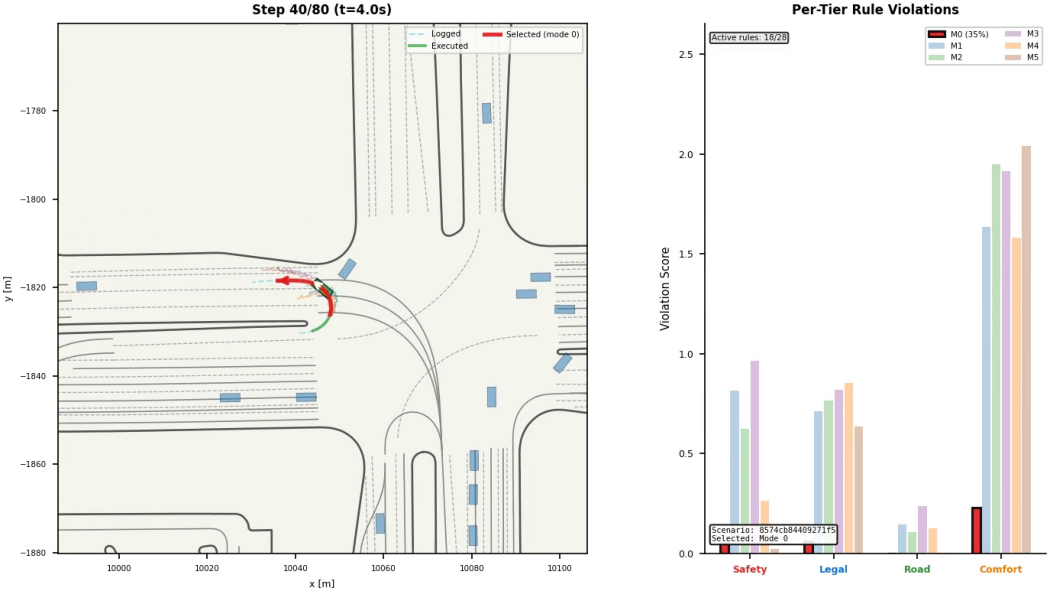
\includegraphics[width=\textwidth]{Figures/scenario_intersection_turn.png}
\caption{Intersection turn}
\end{subfigure}
\hfill
\begin{subfigure}[t]{0.48\textwidth}
\centering
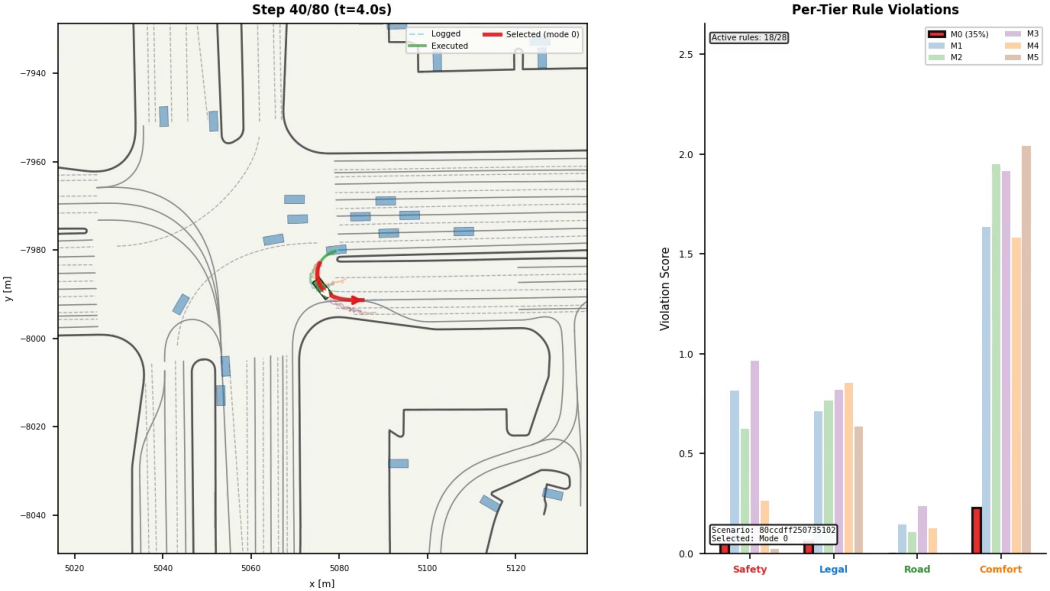
\includegraphics[width=\textwidth]{Figures/scenario_dense_intersection.png}
\caption{Dense intersection}
\end{subfigure}

\vspace{4pt}
\begin{subfigure}[t]{0.48\textwidth}
\centering
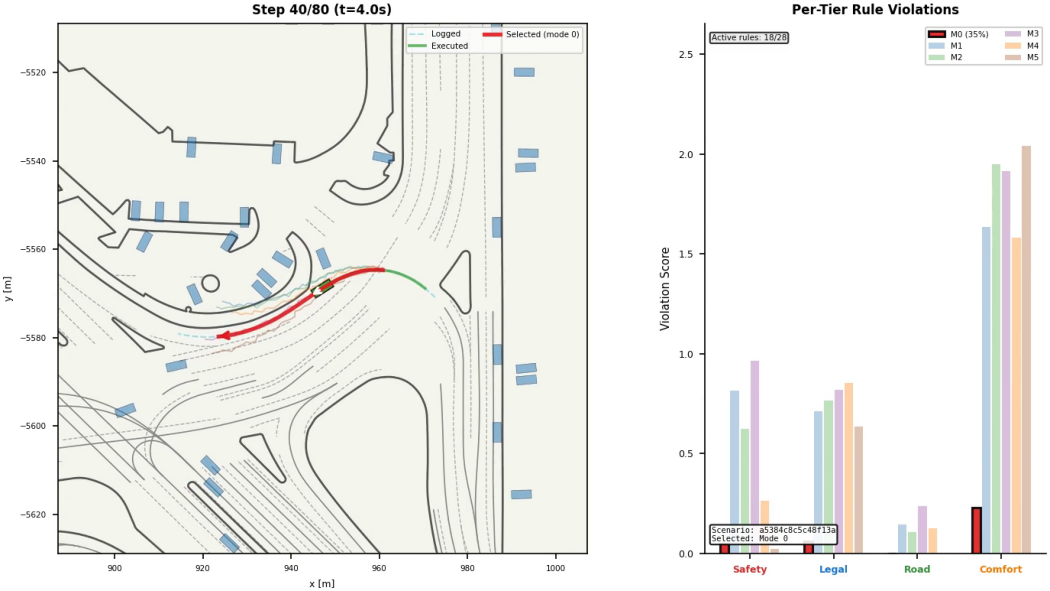
\includegraphics[width=\textwidth]{Figures/scenario_exitramp_merge.png}
\caption{Exit-ramp merge}
\end{subfigure}
\hfill
\begin{subfigure}[t]{0.48\textwidth}
\centering
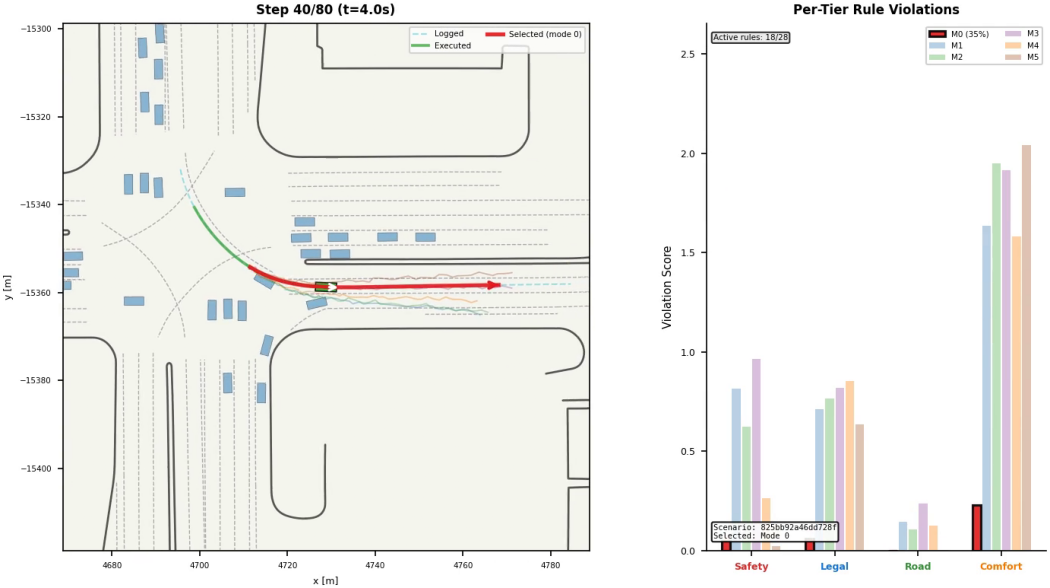
\includegraphics[width=\textwidth]{Figures/scenario_lane_change.png}
\caption{Lane change}
\end{subfigure}

% \vspace{4pt}
% \begin{subfigure}[t]{0.48\textwidth}
% \centering
% 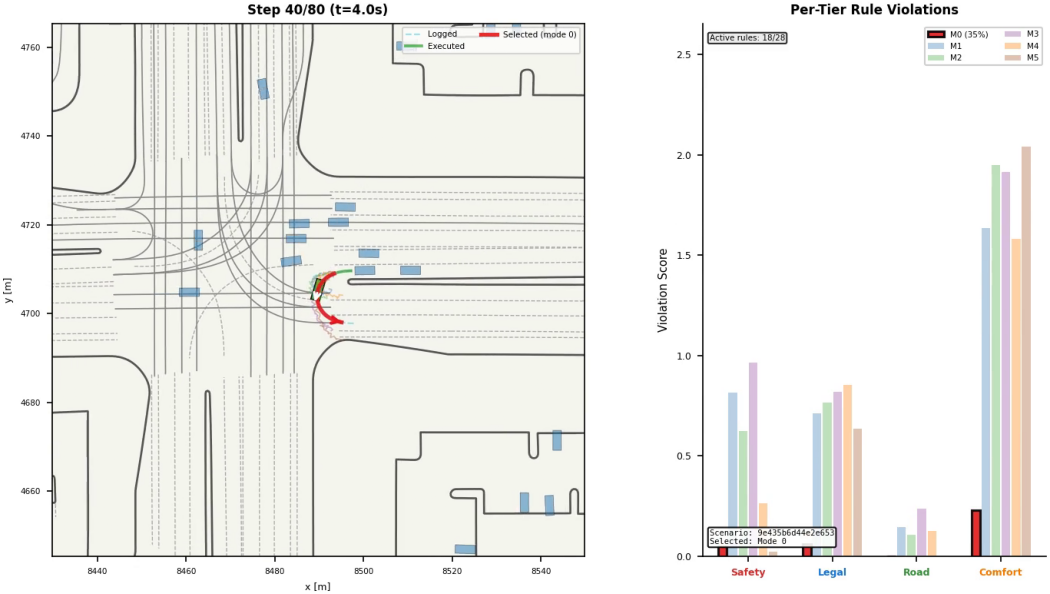
\includegraphics[width=\textwidth]{Figures/scenario_urban_turn.png}
% \caption{Urban turn}
% \end{subfigure}
\caption{Five representative \texttt{validation\_interactive} scenarios from WOMD v1.3.0, rendered from closed-loop Waymax simulation at $t{=}4.1$\,s into the 8-second horizon.  In each panel the BEV map (left) shows surrounding agents (blue rectangles), the RECTOR-selected trajectory (red), and the executed trajectory (green); the bar chart (right) shows per-tier rule violations across the six candidate modes.  The diversity of road geometries and interaction densities reflects the breadth of interactive behaviors used to stress-test the rule-aware selection stack.}
\label{fig:scenario_gallery}
\end{figure*}

\subsubsection{Preprocessing}

Raw TFRecord files are preprocessed into training-ready tensors through five steps:
\begin{enumerate}
    \item \textbf{Coordinate transformation:} all positions are transformed to an ego-centric frame at $t{=}0$.
    \item \textbf{Agent selection:} top 32 agents by proximity to ego.     
    \item \textbf{Lane selection:} top 64 lanes by relevance (proximity and heading alignment).
    \item \textbf{Feature extraction:} velocities are computed via finite differences; accelerations are optionally smoothed for numerical stability.
    \item \textbf{Map tensorisation:} lane polylines, boundaries, stop lines, crosswalks, and drivable surface polygons are vectorised into fixed-size tensors.
\end{enumerate}

\noindent
In addition to standard spatial and temporal augmentations that improve invariances and robustness, we apply rule-targeted augmentation to balance proxy supervision, as summarised in Table~\ref{tab:data_augmentation}.

\begin{table}[h]
\centering
\caption{Data Augmentation Strategies}
\label{tab:data_augmentation}
\begin{tabular}{llp{4cm}}
\toprule
\textbf{Augmentation} & \textbf{Parameters} & \textbf{Purpose} \\
\midrule
Rotation & $\pm 15^\circ$ & Orientation invariance \\
Translation & $\pm 2.0\,\mathrm{m}$ & Position invariance \\
Scaling & $0.95$--$1.05$ & Scale robustness \\
Agent dropout & 10\% prob. & Occlusion handling \\
Trajectory noise & $\mathcal{N}(0, 0.1^2)\,\mathrm{m}$ & Smoothness regularisation \\
Time reversal & 50\% prob. & Temporal symmetry \\
Mirror flip & 50\% prob. & Left-right symmetry \\
\bottomrule
\end{tabular}
\vspace{2mm}
\footnotesize
\textit{Note:} Augmentations are applied in the ego-centric frame.  Agent dropout simulates occlusions; trajectory noise regularises dynamics; mirror flips and rotations improve spatial invariance.  Rule-targeted augmentation generates synthetic samples with controlled violations to balance the proxy
supervision.
\end{table}

To ensure balanced proxy training, we additionally generate synthetic scenarios with controlled violations, including collision perturbations (controlled overlap), speed violations (scaled velocities), lane departures (lateral offsets), and red-light violations (stop-line crossings under red). These samples improve proxy calibration for rare but high-impact events and reduce proxy underfitting on the tail of violation severities.

%-------------------------------------------------------------------------------
\subsection{Summary}
\label{subsec:rule_eval_summary}
%-------------------------------------------------------------------------------

This section defines the 28-rule, four-tier catalog used by RECTOR and describes how compliance is computed under the \emph{Evaluation Dual-Protocol}: Protocol~A applies 24~differentiable proxies with predicted applicability for training and selection, whereas Protocol~B applies the full Waymo evaluator with oracle applicability for reporting and verification.  Per-rule violation breakdowns (Fig.~\ref{fig:rule_breakdown}) expose the dominant failure modes by tier and directly inform proxy refinement, model debugging, and targeted augmentation.  With the rule-evaluation layer and data pipeline fully specified, Section~\ref{Sec:Experiments} next defines the experimental protocol---dataset splits, metrics, and baselines---under which all results are reported.